%!TEX program = xelatex
\documentclass{noiassignment}
\usepackage{cite}
\usepackage{listings}
\usepackage{indentfirst}
\usepackage{ulem}
\usepackage{amsmath}
\usepackage{graphicx}
\usepackage{subfigure}
\usepackage{float}
\usepackage{minted}
\usepackage{fontspec}
\usepackage{xeCJK}
\usepackage{xeCJKfntef}
\usepackage{algorithm}
\usepackage{program}
% \usepackage[]{algorithm2e}
\usepackage{algpseudocode}
% \usepackage{courier}
\usepackage{amsthm,amsfonts,amssymb,bm}
\usepackage{tabularx}
\usepackage{booktabs}
\XeTeXlinebreaklocale "zh"
\XeTeXlinebreakskip = 0pt plus 1pt
\setCJKmainfont{宋体}

\makeatletter
\def\myinline#1#2{%
\ifx\@footnotetext\TX@trial@ftn
\detokenize{#2}%
\else
\mintinline{#1}{#2}%
\fi}
\makeatother

\newtheorem{theorem}{定理}[section]
\newtheorem{definition}[theorem]{定义}
\newtheorem{lemma}[theorem]{引理}
\newtheorem{property}{性质}[theorem]
\newtheorem{corollary}[theorem]{推论}

\usemintedstyle{colorful}
\setminted{obeytabs=true, tabsize=4, xleftmargin=20pt, linenos, fontsize=\footnotesize, breaklines}

\title{Dynamic Memory Allocation}
\author{杨天祺}

\begin{document}
	\maketitle

	\tableofcontents

	\newpage

	\section{摘要}
	由于内存资源有限,但是内核和各个进程都需要使用内存空间,因此内核需要对内存申请进行管理,有效地分配内存空间。

	但是内存分配算法需要考虑的因素比较多,例如算法本身的效率,产生内碎片和外碎片的多少等。但就算不考虑这么多,这个问题也是极其困难的。例如即使我们只考虑最小化一个进程运行的峰值利用率,并且在离线情况下,求解最优的策略也被证明是 NP-Hard 的 \cite{opt-nph}。
	但是在离线情况下,有一些近似算法可以达到较好的复杂度,例如存在一个 $2 + \epsilon$ 近似比的多项式算法 \cite{M2015A},可以较快的得到一个近似解。

	在离线情况下就是 NP-Complete 的,因此在在线的情况下就更加难以处理。一般现在动态内存分配采用贪心思想(例如最先匹配算法),或是一些启发式的方法(例如 slab 算法\cite{bonwick1994slab})等。

	本文前面部分分析了离线情况下最优算法,再对动情况的一些启发式算法做了一些讨论。

	\section{离线问题}
	我们先考虑对于单个程序的离线的情况。这个时候我们提前知道整个内存分配申请序列,要求一个为每一个申请分配的方案,使得某个条件最优化。目前已有研究表明,在最小化申请的堆大小的情况下的求最优解是 NP-Hard 的 \cite{opt-nph},近似算法则有 (2+$\epsilon$) 近似比的多项式算法 \cite{M2015A}。但是对于 NP-Hard 的证明, \cite{opt-nph} 中的证明较为复杂。我们在这里提出一个更为简单的证明。

	\subsection{优化目标}

	这里我们考虑的是最小化峰值利用率 \cite{Bryant:2015:CSP:2846227}。即若我们假定 $n$ 个分配和释放请求按照顺序处理,在处理完第 $i$ 个情况之后,它的有效载荷(payload)是 $P_i$,即当前被分配的所有块的大小和为 $P_i$,而此时堆的大小是 $H_i$。则第 $i$ 个时刻的峰值利用率 $U_i$ 定义为
	$$
	U_i = \frac{\max_{j \le i} P_j}{H_i}
	$$

	我们分配器的目标就是最小化 $U_n$。
	
	而一般我们假设 $H_i$ 是单调不减的,而由于每个时刻我们 $P_i$ 都是确定且已知的,因此 $\displaystyle \max_{i \le n} P_i$ 也是已知的。因此我们最小化 $U_n$,等于最小化 $H_n$。

	\subsection{模型表述}
	
	这个时候我们问题可以被形式化地表述成:
	
	\begin{quotation}
		假定有 $m$ 个单位空间的内存(代表一个大小为 $m$ 的堆)。
		给定 $n$ 个内存分配的申请,第 $i$ 个申请有一个申请大小 $size_i$,以及存在的时间区间 $[tl_i, tr_i]$。
		要为每个内存分配请求分配空间中一个连续的区间 $[l_i, r_i]$,区间长度为 $size_i$,即满足 $r_i - l_i + 1 = size_i$。要求不存在两个分配 $i$ 和 $j$ 满足 $[tl_i, tr_i]$ 和 $[tl_j, tr_j]$ 相交且 $[l_i, r_i]$ 和 $[l_j, r_j]$ 相交。

		求最小的 $m$ 使得存在一个可行的 $[l_i, r_i]$ 序列满足上述条件。
	\end{quotation}

	当然,我们可以二分答案 $m$,变成判断对于一个给定的 $m$,是否存在一个可行的 $[l_i, r_i]$ 序列满足上述条件。

	\subsection{内存分配图}

	我们将每个内存分配请求放到一个二维平面中,这个二维平面中横坐标是时间,纵坐标是 $1 \sim m$ 号内存。那么每个内存分配请求就是一个以 $[tl_i, tr_i]$ 为横坐标区间,$[l_i, r_i]$ 为纵坐标区间的矩形。我们将其称为对应的分配方案的\emph{内存分配图}。
	而内存分配不能冲突的限制就等价与 $n$ 个内存分配请求对应的矩形不相交。而对于每个矩形,$[tl_i, tr_i]$ 是请求的性质,是固定的,而你要求的就是一个可行的 $[l_i, r_i]$ 序列。
	
	例如图 \ref{mm_graph_example} 则为一个可能的内存分配图,这里有 $3$ 个内存分配需求,分别是时刻 $1 \sim 5$ 的一个大小为 $3$ 的申请,时刻 $3 \sim 9$ 的一个大小为 $1$ 的申请,时刻 $6 \sim 11$ 的一个大小为 $3$ 的申请。
	这里将第 $1$ 个申请分配到 $3 \sim 5$ 号内存区域,第 $2$ 个分配到第 $1$ 号,第 $3$ 个分配到第 $2 \sim 4$ 号。此时 $m=5$。当然这不是这个问题的最优答案,因为第 $1$ 个请求我们可以放在 $2 \sim 4$ 的位置,这样 $m$ 就为 $4$。

	\begin{figure}[htbp]
		\centering
		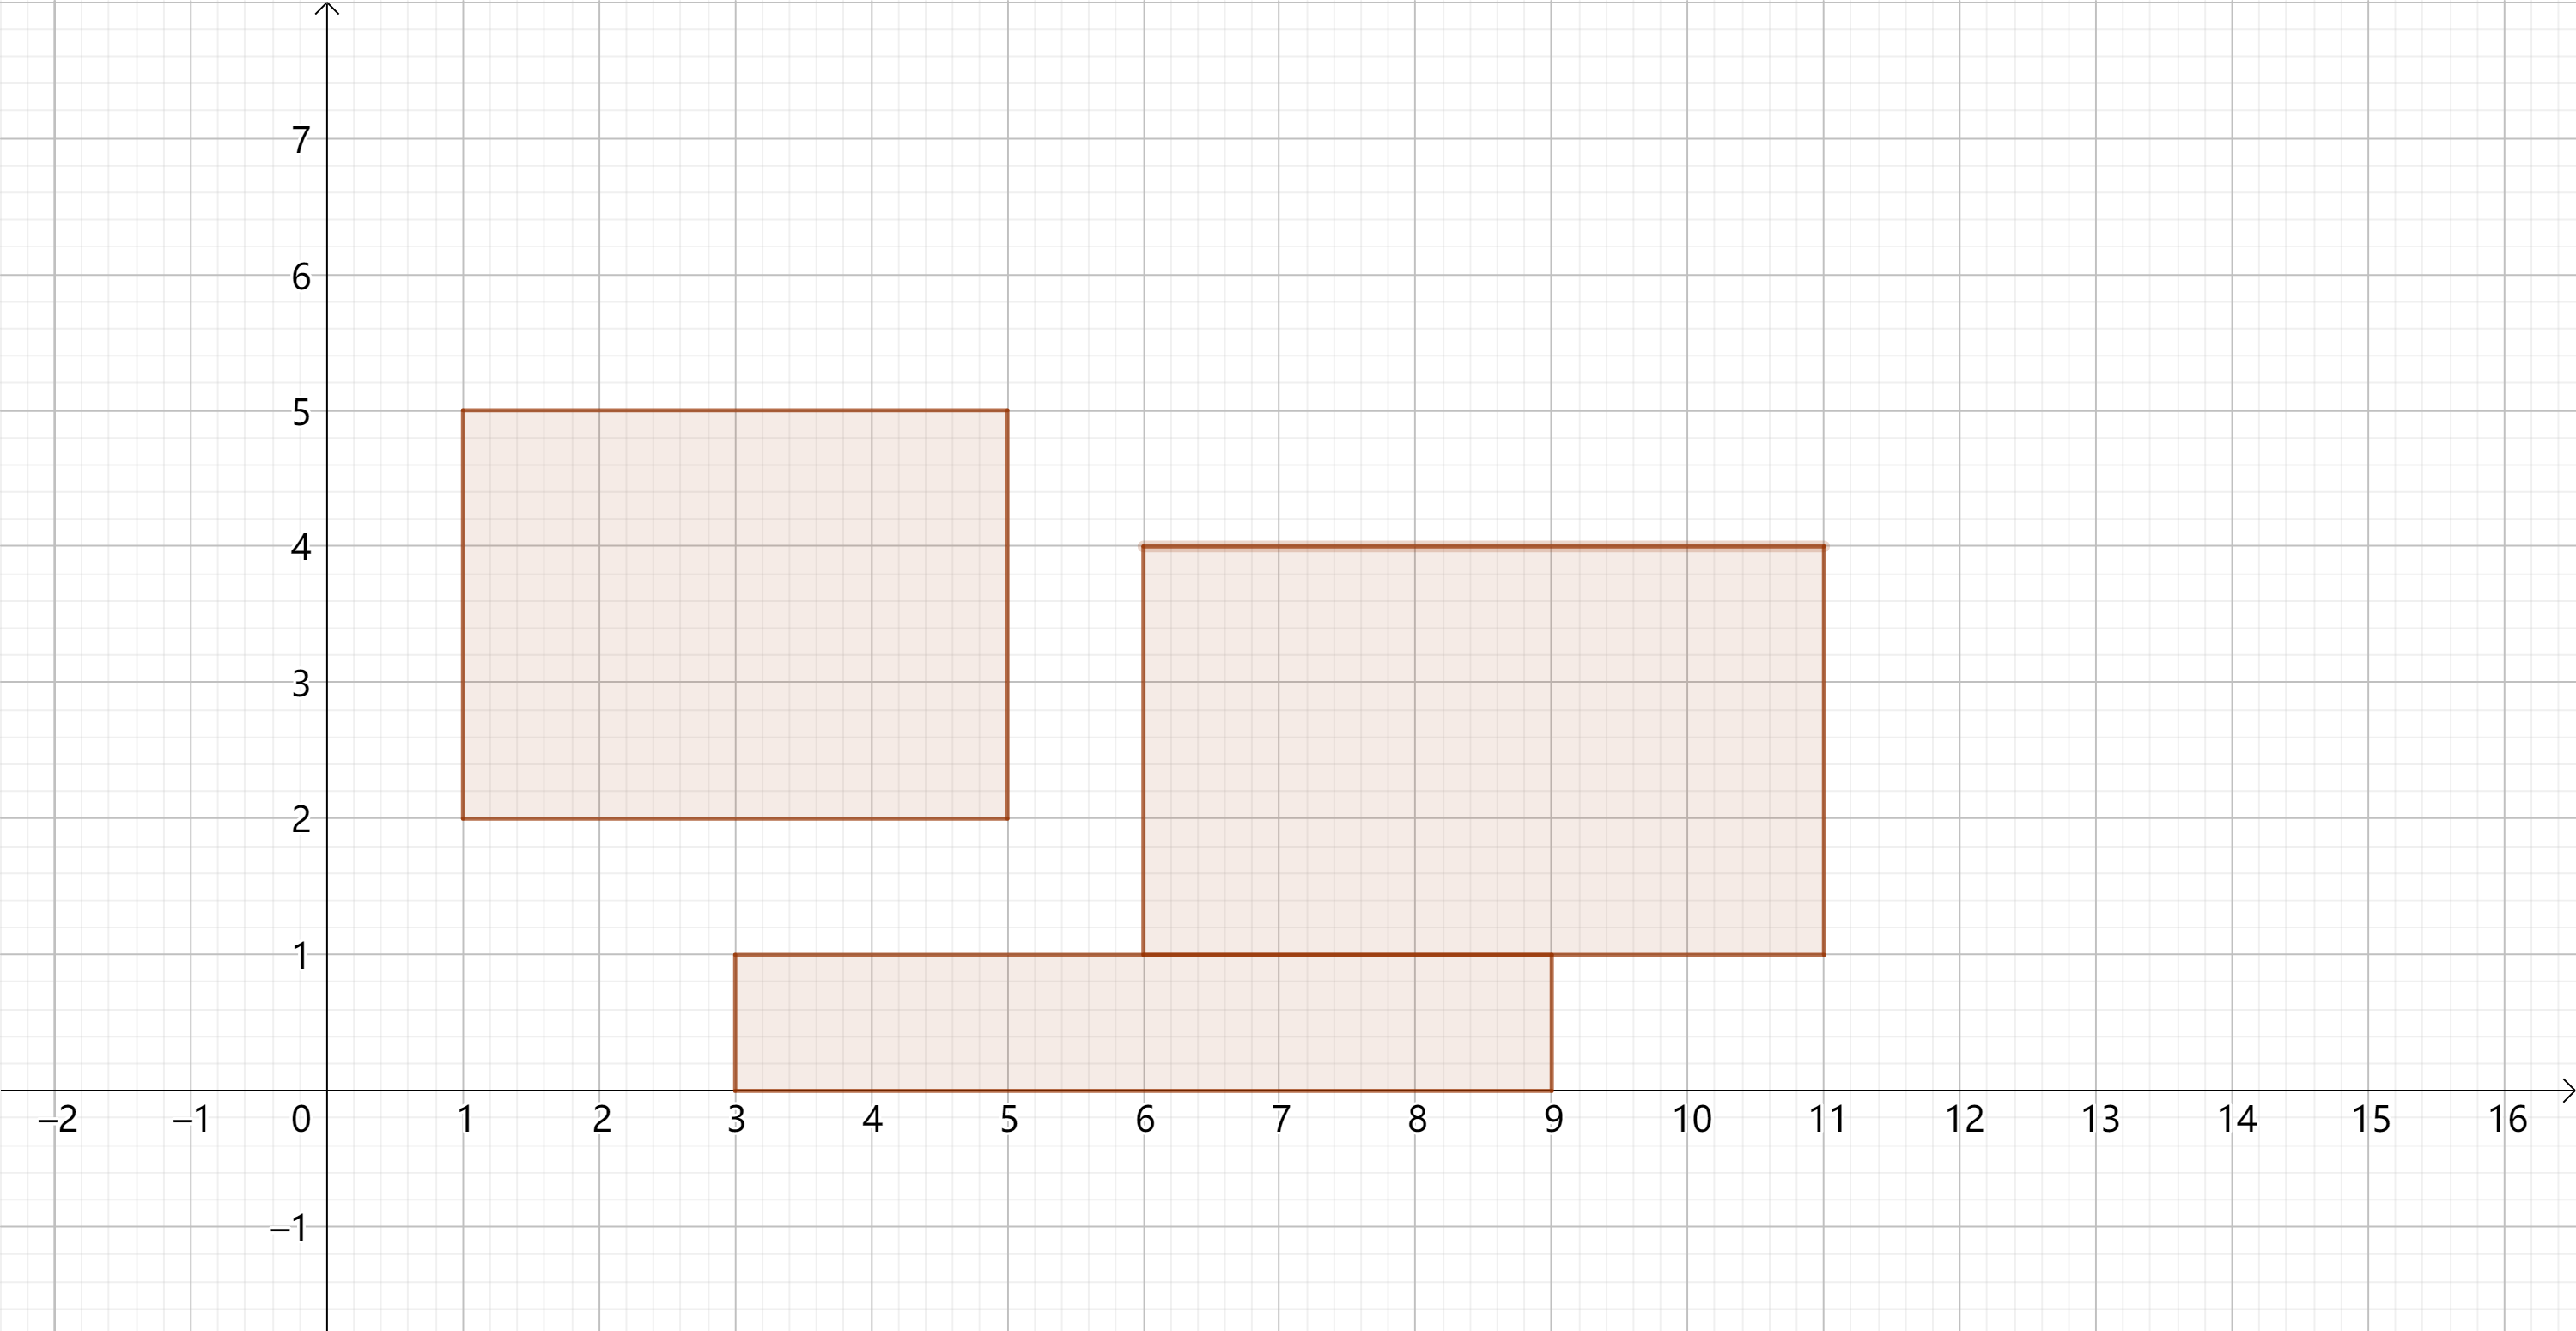
\includegraphics[scale=0.5]{assets/1}
		\caption{内存分配图示例}
		\label{mm_graph_example}
	\end{figure}
	
	因此经过这个转化后,问题变成了如下形式:

	\begin{quotation}
		在二维平面上,给定 $n$ 个矩形,问是否存在一种将所有矩形都上下平移的方案,使得所有矩形的纵坐标都在 $0 \sim m$ 之间,且各个矩形不相交。
	\end{quotation}

	这里上下平移即为选定一个合适的纵坐标起始位置 $l_i$。

	\subsection{最优算法}
	那么最小化峰值利用率就是要求出最小的 $m$,使得存在一个可行的内存分配图。

	\begin{theorem}
		求可行的最小峰值利用率问题是 NP-Complete 的。
	\end{theorem}

	\begin{proof}
		我们尝试将问题规约到 Partition Problem,而 Partition Problem 是 Karp 在 1972 年证明的 $21$ 个 NP-Complete 问题之一 \cite{karp1972reducibility}。

		我们考虑下面这个内存分配图(若有边横坐标相同重合表示它们的先后顺序不影响):
		\begin{figure}[htbp]
			\centering
			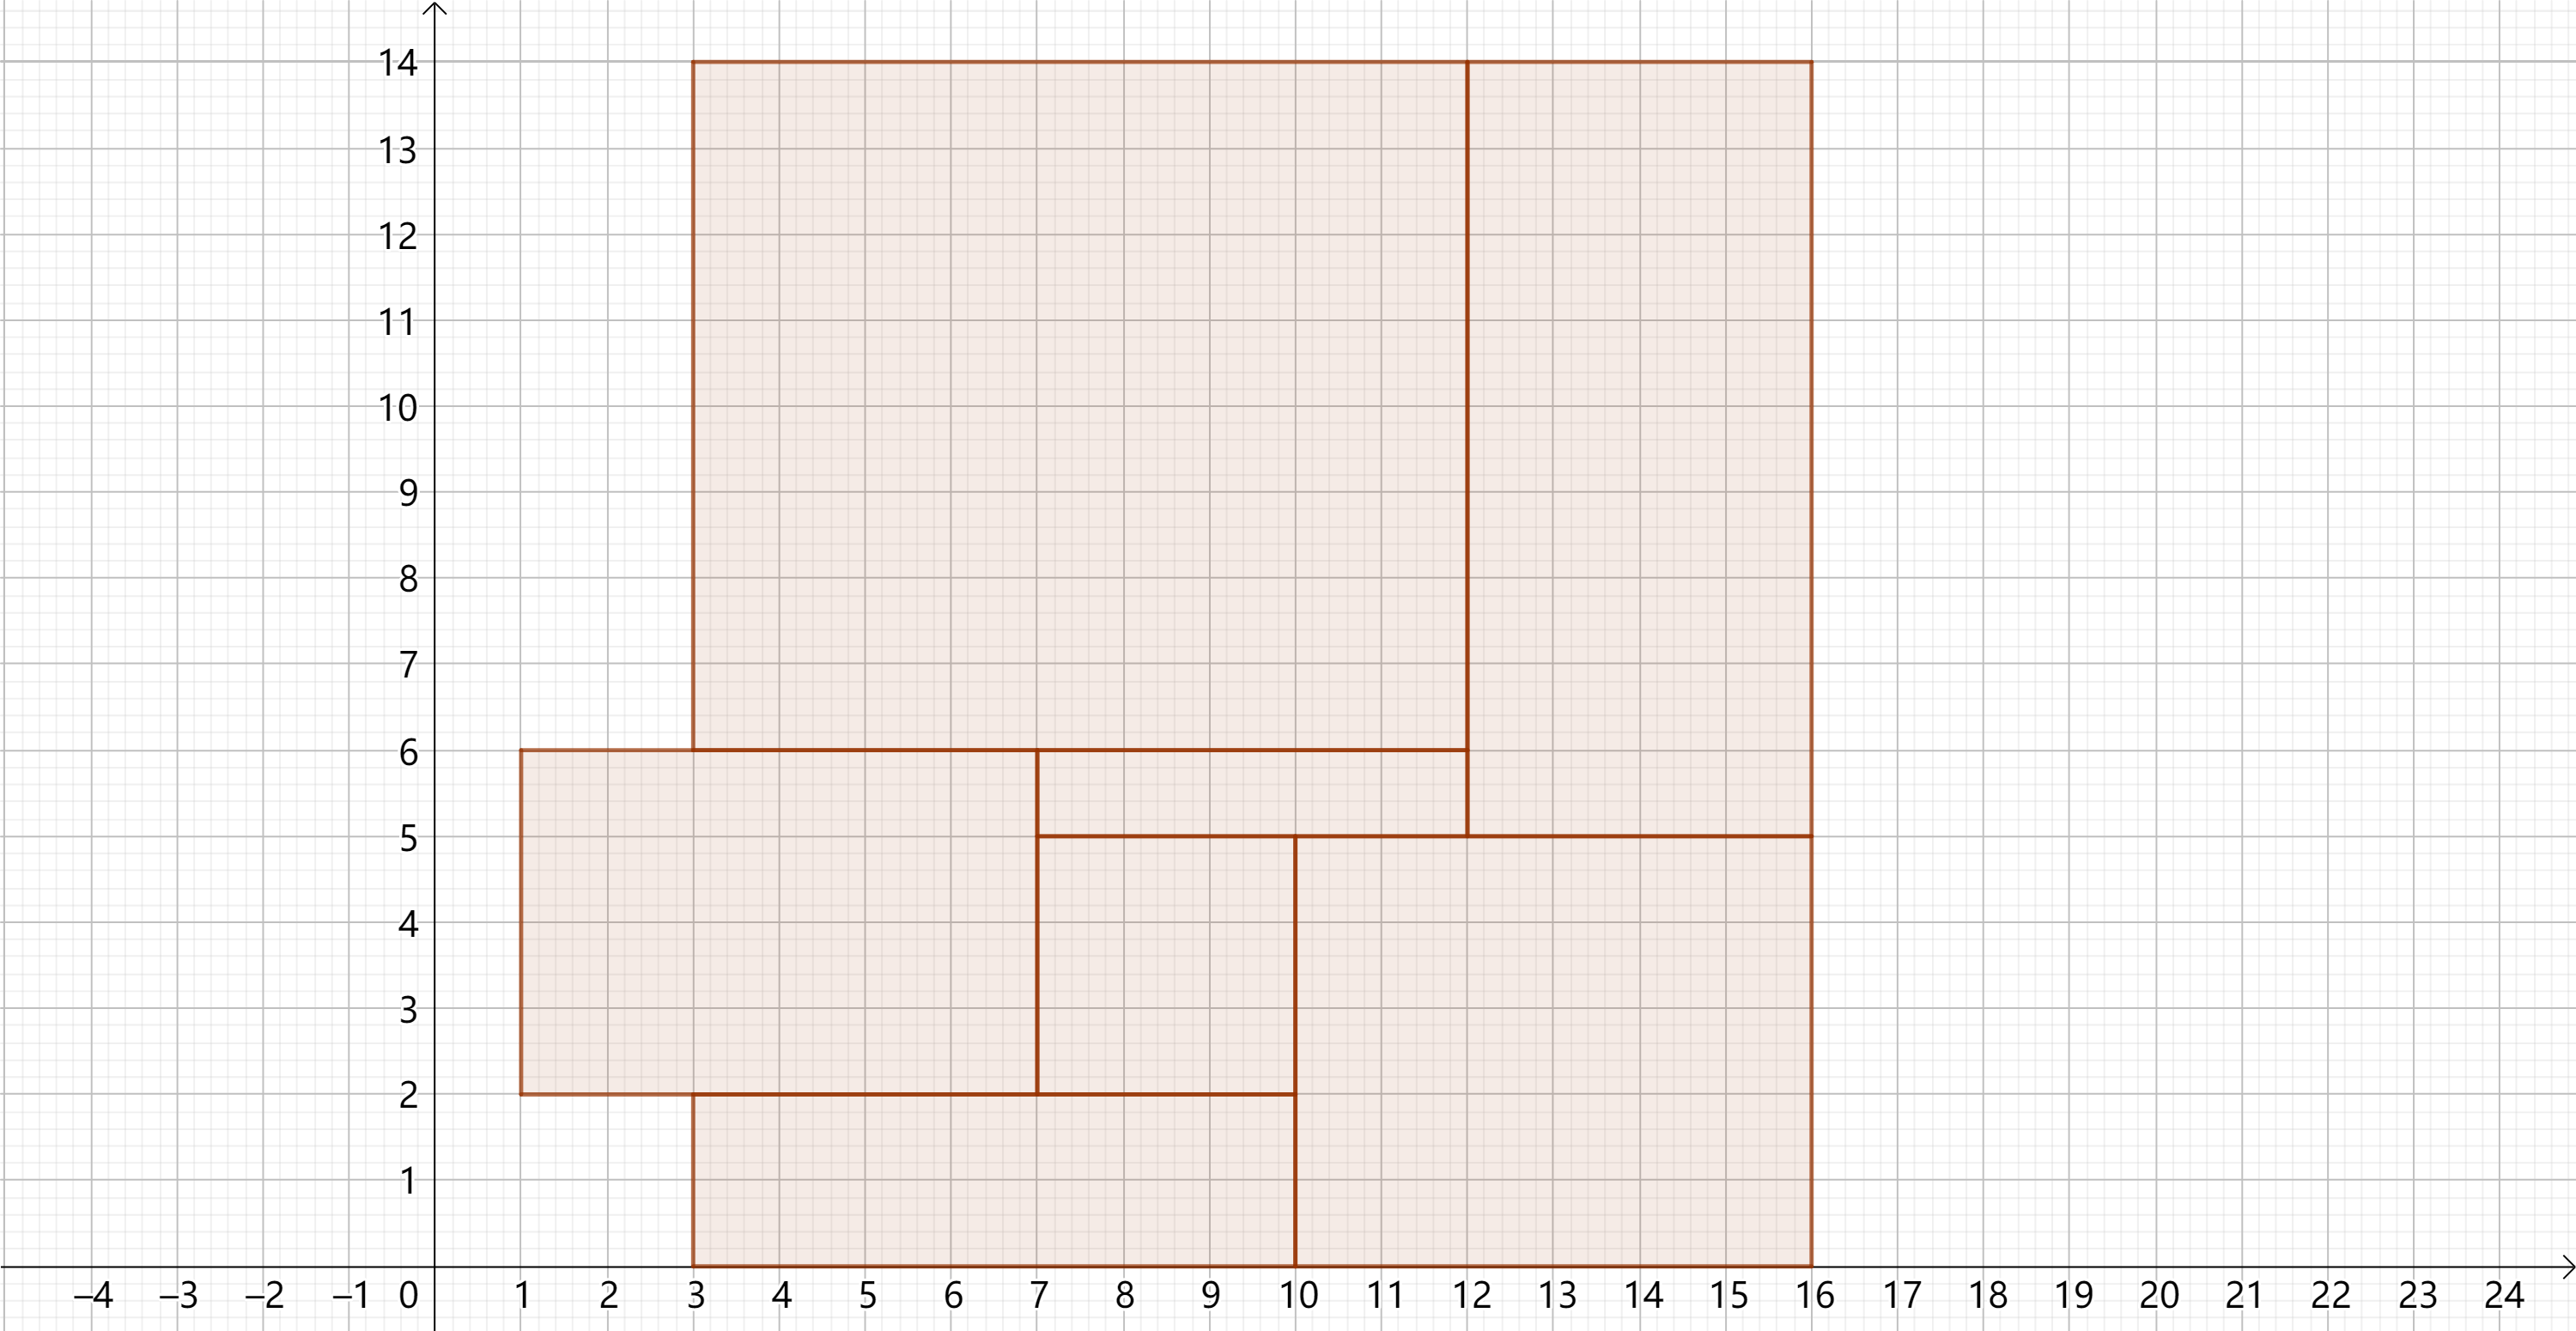
\includegraphics[scale=0.4]{assets/2}
			\caption{构造内存分配图}
			\label{mm_graph_lock}
		\end{figure}

		对于这个内存申请序列而言,可以证明这是唯一的可行的 $m=14$ 的分配方案(除去和它对称的一个)。证明可以通过程序搜索实现。搜索实现可以见 \texttt{tools/opt.cpp}。我们称这张图和其对应的申请序列为 \emph{锁}。
		
		同样可以证明如果把每次申请的内存需求都乘上一个固定的值 $k$,那么也仅存在唯一的 $m=14k$ 的方案,即为将所有矩形纵坐标都乘 $k$ 对应的图。我们称乘 $k$ 之后的结果为 \emph{$k-$锁}。

		那么我们考虑对于一个 Partition Problem,给定一个 $n$ 个元素的集合 $S$,$S$ 中所有元素的和为 $2K$,则我们在 $k-$锁的基础上添加如下一些存在时间在 $[tl_i, tr_i] = [1,2]$ 的内存申请:
		\begin{enumerate}
			\item 一个大小为 $6K$ 的申请
			\item 对于集合 $S$ 中的每个元素 $a$,添加一个大小为 $2a$ 的申请
		\end{enumerate}

		则由于 $6K$ 的申请必须被放在图 \ref{mm_graph_lock} 中最左边的矩形的上面,因此除掉 $6K$ 的申请,剩下的部分被图 \ref{mm_graph_lock} 中最左边的矩形分为上下各 $2K$ 大小的两个部分。
		因此此时我们的问题和将剩下 $S$ 中的每个元素分到上面或下面部分等价。我们要从 $S$ 中选出一个子集,将它们分到下面,剩下的分到上面,而两边选出的集合的和应当都恰好是 $K$。这与 Partition Problem 等价。

		因此我们证明了任何 Partition Problem 都可以用多项式时间转化成我们当前的问题,因此这个问题是 NP-Complete 的。
	\end{proof}

	\section{在线问题}
	由于在线情形我们不知道未来的情况,因此我们只能通过贪心或启发式等方法进行近似。我们可以将动态内存分配算法大致分为以下三类:
	\begin{enumerate}
		\item Sequential-fit Methods,例如最先匹配算法
		\item Buddy Methods,例如 Buddy System
		\item Segregated-storage Methods,例如 Slab
	\end{enumerate}

	\subsection{Sequential-fit Methods}
	这一类算法将所有空闲的块按照一定的方式排序,排成一个线性的结构,然后在 \texttt{alloc} 的时候从线性结构中找出满足条件的第一个块进行分配。这类算法一般采用了贪心策略。一般按照贪心策略的不同分为以下几种:

	\subsubsection{\texttt{First-fit Strategy}}
	这种策略是将所有空闲快按照位置从前向后排序,每次找到第一个足够大的块。这是按照位置从前向后贪心。这种策略实现简单,但是可能会导致前面的位置堆积很多小的外碎片。所需时间会按照分配次数逐渐变长。

	\subsubsection{\texttt{Next-fit Strategy}}
	这是 \texttt{First-fit Strategy} 的一个简易优化。\texttt{First-fit Strategy} 的问题是每次它都从第一个开始找,这会导致靠前的位置容易产生小碎片。因此 \texttt{Next-fit Strategy} 的思路是每次从上一次搜索结束的位置可以找,这样开始位置就具有一定的随机性,避免了碎片的大量堆积。

	\subsubsection{\texttt{Best-fit Strategy}}
	这种策略是将所有空闲块按照大小从小往大排序,每次找到第一个足够大的块。这是按照大小贪心,每次找到最小的可行块。这种策略可以留出更多空间给大的内存申请,但是实现起来相对困难。

	\subsubsection{\texttt{Worst-fit Strategy}}
	这种策略与 \texttt{Best-fit Strategy} 恰好相反,它把所有空闲块按从大向小排序,每次找到最大的一块。这个方法在申请较多小内存的时候较有用。

	\subsection{Buddy Methods}
	这部分比较常用的即为 Buddy Memory Allocation,思路是将内存每次分成两块,然后按照二进制进行分配。详情可以参见 \cite{wiki:buddy}。

	\newpage

	\bibliography{ref}
	\bibliographystyle{plain}
\end{document}
